We can place an upper limit on the contribution of metallicity to the measured PL dispersion by combining the probability distributions of the known intrinsic PL width and the scatter induced by photometric error and comparing the result to the observed distribution of $\omega$~Cen PL residuals. The following description of the process uses the RRab PL relation in [3.6] as the example case; we apply this method to both pulsation modes in both IRAC filters, with results presented in Table~\ref{tab:metallicity_sigma}. We model the intrinsic scatter as a uniform distribution with an area of 1 and full $12\sigma$ width of $\sqrt{12}$ times the intrinsic PL width (see Table~\ref{tab:pl_table_m4}), $\sqrt{12} \times 0.040 = 0.139$ mag and the photometric uncertainties as a unit area Gaussian distribution with a standard deviation of the mean photometric error in the sample, $\sigma = 0.048$ mag. We model the probability distribution of the observed PL residuals as a unit area Gaussian centered at zero with a scale of the standard deviation of the residuals, $\sigma = 0.088$ mag. These models are shown in Figure~\ref{fig:probdist1}, as well as the convolution of the intrinsic scatter and photometric error distributions.

\begin{figure}
\begin{center}
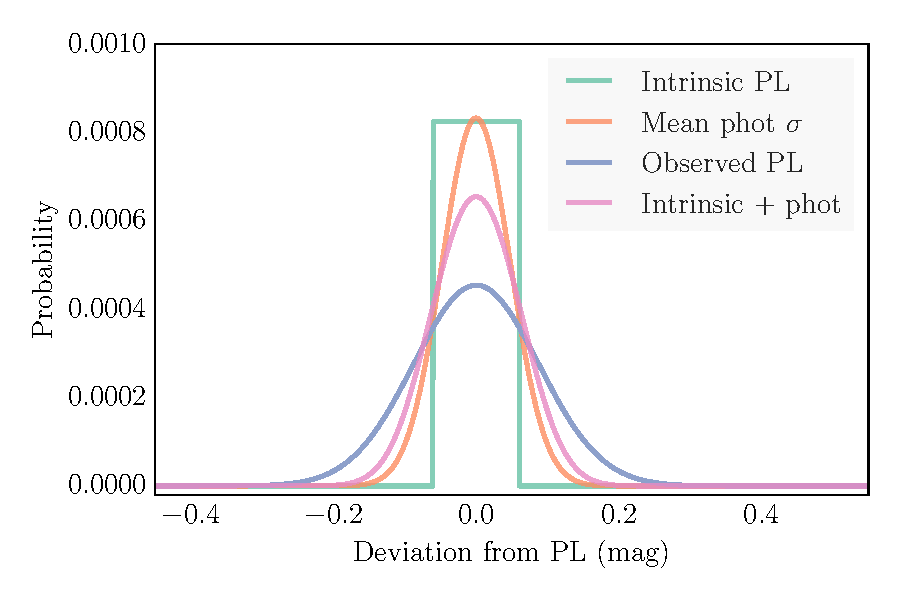
\includegraphics[width=80mm]{reworked_fitting_code/final_plots/distributions_nofeh_ab_3_gaussian.pdf}
\caption{Probability distributions for components of PL scatter for RRab's in [3.6], with intrinsic width in green, photometric error in orange, the combination thereof in purple, and the observed distribution in pink.}
\label{fig:probdist1}
\end{center}
\end{figure}

To constrain the contribution of metallicity to the observed scatter, we model the metallicity-induced scatter as another Gaussian centered at zero. To find the standard deviation of this model, we convolve the metallicity distribution with the previous convolution of the intrinsic width and photometric error distributions, and minimize the difference between that and the observed distribution. For RRab's in [3.6], we find the standard deviation of the model metallicity distribution to be $\sigma = 0.061$, as shown in Figure~\ref{fig:probdist2}. The results for all IRAC PLs are in Table~\ref{tab:metallicity_sigma}.

\begin{figure}
\begin{center}
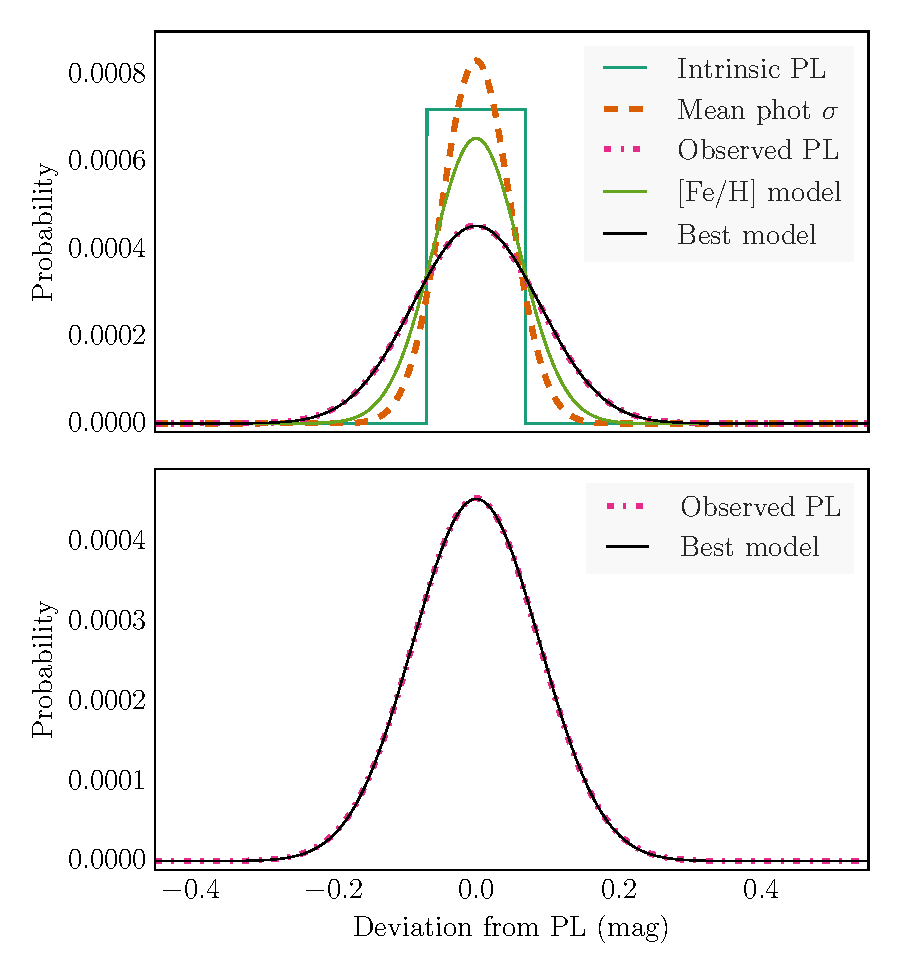
\includegraphics[width=80mm]{reworked_fitting_code/final_plots/distributions_ab_3_gaussian.pdf}
\caption{Top: Intrinsic, photometric error, and observed PL relations for RRab's in [3.6] as in Figure~\ref{fig:probdist1}, as well as the scaled metallicity distribution and best model (convolution of intrinsic, photometric, and metallicity distributions). Bottom: only the observed and model distributions for easier comparison.}
\label{fig:probdist2}
\end{center}
\end{figure}

\begin{table}
\centering
\caption{The standard deviation of the observed spread of the PL residuals $\sigma_{\text{observed}}$ ($\sigma_{\text{PL}}$ in Table~\ref{tab:dist_mod}) and its components: $\sigma_{\text{intrinsic}}$ ($\sigma$ in Table~\ref{tab:pl_table_m4}), $\sigma_{\text{phot}}$, and $\sigma_{[\text{Fe/H}]}$ for all IRAC PL relations.}
\label{tab:metallicity_sigma}
\begin{tabular}{lccccr} 
\hline \hline
Band & Mode & $\sigma_{\text{observed}}$ & $\sigma_{\text{intrinsic}}$ & $\sigma_{\text{phot}}$ & $\sigma_{[\text{Fe/H}]}$ \\
\hline
$[3.6]$ & RRab & 0.088 & 0.040 & 0.048 & $0.061$ \\ % & $0.282$ & $0.234$\\
$[3.6]$ & RRc & 0.102 & 0.079 & 0.041 & $0.046$ \\ %& $0.778$ & $0.323$\\
$[4.5]$ & RRab & 0.173 & 0.045 & 0.046 & $0.160$ \\ % & $0.712$ & $0.590$\\
$[4.5]$ & RRc & 0.202 & 0.057 & 0.048 & $0.187$ \\ %& $1.660$ & $0.689$\\
\hline
\end{tabular}
\end{table}

We use these measurements to assess the $\gamma$ parameter for $\omega$~Cen, where 
\begin{equation} \label{eqn:gamma}
\gamma = \dfrac {\Delta \text{mag}} {\Delta [\text{Fe/H}]}\text{,}
\end{equation}
similar to $\gamma$ used to quantify the effect of metallicity on the zero-point of the Cepheid PL relation \citep{1998ApJ...498..181K, 2009MNRAS.396.1287S}. Here we calculate $\gamma$ by dividing the standard deviation of the metallicity component of the PL scatter by the standard deviation of the metallicity values; the results for each PL are shown in Table~\ref{tab:gamma}. We use all available metallicity values for each pulsation mode when taking the standard deviation, as we do not have metallicity values for all stars in our samples, although the ones we do have trace the overall metallicity distributions fairly well (see Figure~\ref{fig:metallicity_hists}).

\begin{table}
\centering
\caption{Metallicity standard deviations and $\gamma$ values.}
\label{tab:gamma}
\begin{tabular}{lccccr} 
\hline \hline
Band & Mode & $\sigma_{\text{[Fe/H]spect}}$ & $\sigma_{\text{[Fe/H]phot}}$ & $\gamma_{\text{spect}}$ & $\gamma_{\text{phot}}$ \\
\hline
$[3.6]$ & RRab & 0.250 & 0.254 & 0.244 & 0.240 \\ % & $0.282$ & $0.234$\\
$[3.6]$ & RRc & 0.132 & 0.243 & 0.349 & 0.189 \\ %& $0.778$ & $0.323$\\
$[4.5]$ & RRab & 0.250 & 0.254 & 0.642 & 0.632 \\ % & $0.712$ & $0.590$\\
$[4.5]$ & RRc & 0.132 & 0.243 & 1.420 & 0.771 \\ %& $1.660$ & $0.689$\\
\hline
\end{tabular}
\end{table}
